\documentclass{article}
\usepackage{graphicx}
\usepackage{subcaption}
\usepackage{wrapfig}

\begin{document}

% graphicx宏包命令
%picture in the same file as Tex
% 图片原始大小
\includegraphics{doraemon1.jpg}
% XeLaTeX支持pdf、eps、png与jpg图片扩展名,所以可以写带扩展名的图片名称,也可以写不带扩展名的名称,如果不给出扩展名,将按上述4个扩展名的顺序依次搜索文件(吴康隆P50)

% 绝对路径
% \includegraphics{D:/OneDrive/(▲)Yuanhao_github/Yuanhao_LaTeX_github/Test/LaTeX_Picture/doraemon1.jpg} 
%? 使用相对路径始终无法成功编译,不知道原因是什么

%reserved file for pictures
% \graphicspath{{D:/OneDrive/(▲)Yuanhao_github/Yuanhao_LaTeX_github/Test/LaTeX_Picture/Reserved file for pictures}}
% 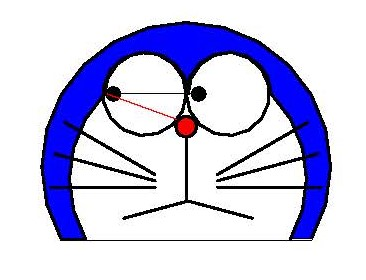
\includegraphics{doraemon2.jpg}
%* 注意,使用"\graphicspath{dir-list}"命令时,路径两边应该套用两层大括号,否则无法成功编译

% scale表示图片缩放倍数
\includegraphics[scale=.3]{doraemon1.jpg}
\includegraphics[scale=.5]{doraemon1.jpg}
\includegraphics[scale=.7]{doraemon1.jpg}

% width表示图片宽度
\includegraphics[width=3cm]{doraemon1.jpg}
\includegraphics[width=.3\textwidth]{doraemon1.jpg}

% height表示图片高度
% 旋转的图片基线会变化,故一般用totalheight代替height(吴康隆P50)
\includegraphics[height=1cm]{doraemon1.jpg}
\includegraphics[height=.1\textheight]{doraemon1.jpg}

% angle表示图片逆时针旋转角度
%* 顺时针旋转可以通过在旋转角度前面添加符号来完成
% origin表示图片旋转中心,默认值为l(左),可以设置为r(右)、c(中)、t(顶)、b(底)、B(基线)
\includegraphics[scale=.3, angle=90]{doraemon1.jpg}%counterclockwise
\includegraphics[scale=.3, angle=-90]{doraemon1.jpg}%clockwise
\includegraphics[scale=.3, angle=90, origin=c]{doraemon1.jpg}%counterclockwise
\includegraphics[scale=.3, angle=-90, origin=c]{doraemon1.jpg}%clockwise

\fbox{\includegraphics{doraemon1.jpg}}
\setlength{\fboxsep}{.5cm}
\fbox{\includegraphics{doraemon1.jpg}}

This is a picture \includegraphics{doraemon1.jpg} inserted into the text.

This is a picture independent of the text.
\begin{figure}[htbp]
    \centering
    \includegraphics{doraemon1.jpg}
    \caption{doraemon}
\end{figure}

% subcaption宏包命令
\begin{figure}[htbp]
    \centering
	\begin{subfigure}{.3\textwidth}%this argument of width is obligatory
        \centering
        \includegraphics[scale=.1]{doraemon1.jpg}
        \subcaption{doraemon (1)}
	\end{subfigure}
	%
	\begin{subfigure}{.3\textwidth}
        \centering
        \includegraphics[scale=.3]{doraemon1.jpg}
        \subcaption{doraemon (2)}
	\end{subfigure}
	%
	\begin{subfigure}{.3\textwidth}
        \centering
        \includegraphics[scale=.5]{doraemon1.jpg}
        \caption{doraemon (3)} % subfigure环境中既可以使用"\subcaption{}"命令,也可以使用"\caption{}"命令
	\end{subfigure}	
    \caption{subfigure}	
\end{figure}

% wrapfig宏包命令
\begin{wrapfigure}{l}{5cm}%Notice that this is the argument of width 
    \centering
    \includegraphics[scale=.3]{doraemon1.jpg}
    \caption{picture inserted}
\end{wrapfigure}
Texte texte texte texte texte texte texte
texte texte texte texte texte texte texte
texte texte texte texte texte texte...
Texte texte texte texte texte texte texte
texte texte texte texte texte texte texte
texte texte texte texte texte texte...
Texte texte texte texte texte texte texte
texte texte texte texte texte texte texte
texte texte texte texte texte texte...

\clearpage
\listoffigures
\end{document}